\documentclass[11pt,a4paper]{article}
\usepackage[UTF8]{ctex}
\usepackage{graphicx}
\usepackage{amsmath,amssymb}
\usepackage{booktabs}
\usepackage{multirow}
\usepackage{array}
\usepackage{float}
\usepackage{hyperref}
\usepackage{listings}
\usepackage{xcolor}
\usepackage{subcaption}
\usepackage[a4paper,margin=2.5cm]{geometry}
\usepackage{enumitem}
\usepackage{url}
\usepackage{natbib}
\usepackage{fancyhdr}

\pagestyle{fancy}
\fancyhf{}
\fancyhead[C]{Self-RAG 复现与改进实验报告}
\fancyfoot[C]{\thepage}

\lstset{
    language=Python,
    basicstyle=\footnotesize\ttfamily,
    breaklines=true,
    frame=single,
    keywordstyle=\color{blue},
    commentstyle=\color{teal},
    stringstyle=\color{red!70!black}
}

\title{\bf 自然语言处理课程报告\\[0.5em]
\Large Self-RAG: 自反思检索增强生成的复现与改进}
\author{姓名：\underline{~~~~~~~~~叶盛豪~~~~~~~~~} \quad 学号：\underline{~~~~~PB24000227~~~~~~}}
\date{\today}

\begin{document}
\maketitle

\begin{abstract}
检索增强生成（Retrieval-Augmented Generation, RAG）是提升大语言模型事实准确性的重要范式，但传统 RAG 方法存在不加区分地检索外部文档、无法判断检索结果质量等问题。Self-RAG 通过引入反思 Token（Reflection Tokens）机制，使语言模型能够在推理过程中自主决定是否检索、评估检索段落的相关性与支持度，并对生成结果进行自我批判。

本报告对 Self-RAG 进行了系统性的复现与改进实验。在复现阶段，我们基于 Llama-2-7B 成功训练了 Critic 和 Generator 模型，在 PopQA、ARC-Challenge 和 TriviaQA 三个数据集上的评测结果与原论文保持一致。在改进阶段，我们完成了三项工作：（1）消融实验揭示了 Groundness 评分机制是检索增强的核心贡献因子（贡献 4.22 个百分点），而 Utility 评分对短答案 QA 任务影响甚微；（2）将 Self-RAG 框架迁移至 Qwen2.5-7B 基座，验证了方法的跨架构泛化能力；（3）构建了基于 Gradio 的交互式 Demo 系统。此外，我们详细记录了 21 项工程问题及其解决方案，为后续研究提供了实践参考。

\noindent\textbf{关键词}：检索增强生成；反思 Token；Self-RAG；消融实验；大语言模型
\end{abstract}

% ================================================================
\section{引言}
\label{sec:intro}

大语言模型（Large Language Models, LLMs）在自然语言处理的众多任务上取得了显著进展，但其核心局限之一在于\textbf{幻觉}（Hallucination）——模型可能生成看似流畅但事实错误的内容。这一问题在知识密集型任务（如开放域问答）中尤为突出，因为模型的参数化知识不可避免地存在时效性和覆盖范围的限制。

检索增强生成（RAG）通过在推理时引入外部检索器来缓解这一问题：模型先从知识库中检索相关文档，再基于检索结果生成回答。然而，传统 RAG 方法存在以下不足：
\begin{enumerate}[leftmargin=2em]
    \item \textbf{无差别检索}：对所有输入查询一律执行检索，即使模型内部已拥有足够的知识来回答问题（如"法国的首都是什么"），也会引入不必要的计算开销和检索噪声；
    \item \textbf{缺乏质量判断}：模型无法评估检索到的段落是否真正支持所生成的回答，可能导致"检索了但没用对"的困境；
    \item \textbf{端到端优化困难}：检索器和生成器通常是独立训练的，二者之间缺乏有效的反馈机制。
\end{enumerate}

Asai 等人 (2024) 提出的 \textbf{Self-RAG}（Self-Reflective Retrieval-Augmented Generation）从根本上改变了 RAG 的范式。其核心创新在于引入了一组\textbf{反思 Token}（Reflection Tokens），使语言模型在生成过程中能够：（1）自主判断当前是否需要检索（\texttt{[Retrieval]} / \texttt{[No Retrieval]}）；（2）评估检索段落的相关性（\texttt{[Relevant]} / \texttt{[Irrelevant]}）；（3）判断生成内容是否被检索证据支持（\texttt{[Fully supported]} / \texttt{[Partially supported]}）；（4）对最终输出的整体质量进行评分（\texttt{[Utility:1-5]}）。

本报告的主要贡献包括：
\begin{itemize}[leftmargin=2em]
    \item 在单卡 NVIDIA A40 (48GB) 上完整复现了 Self-RAG 的 Critic 和 Generator 训练流程，并在 PopQA、ARC-C、TriviaQA 三个基准上验证了复现结果与原论文的一致性；
    \item 通过消融实验定量分析了各反思 Token 评分机制的独立贡献，发现 Groundness 评分是检索增强有效性的关键因子；
    \item 将 Self-RAG 框架成功迁移至 Qwen2.5-7B 基座模型，验证了方法的跨架构泛化能力；
    \item 构建了基于 Gradio + vLLM 的交互式 Demo 系统，直观展示反思 Token 的推理行为；
    \item 系统记录了 21 项工程实践问题及解决方案，涵盖显存优化、数据处理、跨架构兼容等方面。
\end{itemize}

% ================================================================
\section{相关工作}
\label{sec:related}

\textbf{检索增强生成（RAG）。}Lewis 等人 (2020) 提出的 RAG 模型将预训练语言模型与稀疏/稠密检索器相结合，在开放域 QA 上取得了显著提升。后续工作如 REALM (Guu et al., 2020)、Atlas (Izacard et al., 2023) 进一步优化了检索器与生成器的联合训练。然而，这些方法通常对所有查询执行统一检索，缺乏按需检索的灵活性。

\textbf{自适应检索。}部分工作探索了让模型自主决定是否检索的机制。FLARE (Jiang et al., 2023) 通过检测低置信度 Token 来触发检索；Self-RAG 则通过训练模型生成显式的检索决策 Token，实现了更精细的自适应控制。

\textbf{自我批判与反思。}Constitutional AI (Bai et al., 2022) 和 Self-Refine (Madaan et al., 2023) 让模型对自身输出进行批判和迭代修正。Self-RAG 将这一思想内化为词表中的反思 Token，使模型在单次前向传播中即可完成生成与自我评估。

% ================================================================
\section{Self-RAG 方法概述}
\label{sec:method}

Self-RAG 的核心思想是将检索决策和质量评估内化为语言模型的生成过程。具体而言，模型的词表在原始 Token 基础上扩展了一组反思 Token，模型在自回归生成中穿插生成这些特殊 Token，实现对自身行为的元认知控制。整个框架包含两个模型的训练和一套推理流程。

\subsection{反思 Token 机制}
\label{sec:tokens}

Self-RAG 定义了四类共 15 个反思 Token，如表~\ref{tab:tokens}~所示。

\begin{table}[H]
\centering
\caption{Self-RAG 反思 Token 定义}
\label{tab:tokens}
\begin{tabular}{p{2.5cm}p{4cm}p{6cm}}
\toprule
类别 & Token & 语义 \\
\midrule
检索决策 & \texttt{[Retrieval]} / \texttt{[No Retrieval]} & 模型判断当前是否需要检索外部文档 \\
\midrule
相关性评估 & \texttt{[Relevant]} / \texttt{[Irrelevant]} & 检索到的段落是否与查询相关 \\
\midrule
支持度评估 & \texttt{[Fully supported]} / \texttt{[Partially supported]} / \texttt{[No support / Contradictory]} & 生成内容是否被检索证据支持（Groundness） \\
\midrule
效用评分 & \texttt{[Utility:1]} $\sim$ \texttt{[Utility:5]} & 生成结果对原始查询的整体有用性 \\
\bottomrule
\end{tabular}
\end{table}

这些 Token 被添加到模型词表中（将词表从 32,000 扩展到 32,016），在训练数据中作为标注信号出现，模型学习在合适的位置生成它们。

\subsection{训练流程}
\label{sec:training_pipeline}

Self-RAG 的训练分为两阶段：

\textbf{阶段一：Critic 模型训练。}使用 GPT-4 对训练数据中的检索段落和生成文本进行多维度标注（相关性、支持度、效用），得到约 48.5K 条标注数据。基于 Llama-2-7B 基座，以分类任务的形式训练 Critic 模型，使其学会预测各类反思 Token。训练损失函数为标准的交叉熵：
\begin{equation}
\mathcal{L}_{\text{critic}} = -\sum_{t} \log P(y_t^{\text{reflect}} \mid x, y_{<t})
\end{equation}

\textbf{阶段二：Generator 模型训练。}使用训练好的 Critic 对大规模指令微调数据进行自动标注，得到约 145K 条带反思 Token 的训练数据。同样基于 Llama-2-7B，以标准的因果语言模型目标训练 Generator，使其学会在生成文本的同时穿插生成反思 Token：
\begin{equation}
\mathcal{L}_{\text{gen}} = -\sum_{t} \log P(y_t \mid x, y_{<t}), \quad y_t \in \mathcal{V} \cup \mathcal{V}_{\text{reflect}}
\end{equation}
其中 $\mathcal{V}$ 为原始词表，$\mathcal{V}_{\text{reflect}}$ 为 16 个反思 Token。

\subsection{推理流程}
\label{sec:inference}

推理时，Self-RAG 支持两种模式：

\textbf{No Retrieval 模式}：模型直接基于内部参数化知识生成回答。如果模型生成了 \texttt{[Retrieval]} Token，表明其认为需要外部信息，但在此模式下不执行检索。

\textbf{Always Retrieve 模式}：对每个查询，从预检索的段落集合中选取 top-$k$ 段落（本实验取 $k=5$），模型为每个段落独立生成候选回答。随后使用 Groundness 和 Utility 评分对候选回答进行排序，选出最优输出：
\begin{equation}
\text{score}(y \mid d) = w_g \cdot P(\texttt{[Fully supported]} \mid y, d) + w_u \cdot P(\texttt{[Utility:5]} \mid y)
\end{equation}
其中 $w_g$ 和 $w_u$ 分别为 Groundness 和 Utility 的权重系数。

% ================================================================
\section{实验设置}
\label{sec:setup}

\subsection{硬件环境}

\begin{table}[H]
\centering
\caption{实验硬件与软件环境}
\begin{tabular}{ll}
\toprule
配置项 & 详情 \\
\midrule
GPU & NVIDIA A40 (48GB VRAM) $\times$ 8 (使用单卡) \\
CPU & Intel Xeon Gold 6330 (56 cores) \\
内存 & 1TB DDR4 \\
PyTorch & 2.4.0 + CUDA 12.4 \\
推理引擎 & vLLM 0.5.5 \\
Python & 3.10.20 (Conda 隔离环境) \\
\bottomrule
\end{tabular}
\end{table}

所有训练和推理均在单卡 A40 上完成。训练时使用 Adafactor 优化器（替代 AdamW 以节省约 12GB 优化器状态显存）和 Gradient Checkpointing，总显存占用约 40--44GB。

\subsection{数据集}

\textbf{训练数据：}
\begin{itemize}[leftmargin=2em]
    \item \textbf{Critic 训练集}：约 48.5K 条，由 GPT-4 标注的多维度反思 Token 标签；
    \item \textbf{Generator 训练集}：约 145K 条，由训练好的 Critic 自动标注的带反思 Token 的指令微调数据。
\end{itemize}

\textbf{评测数据：}

\begin{table}[H]
\centering
\caption{评测数据集统计}
\label{tab:eval_data}
\begin{tabular}{lccp{6cm}}
\toprule
数据集 & 样本数 & 指标 & 任务描述 \\
\midrule
PopQA & 1,399 & Accuracy (match) & 长尾实体知识 QA，每条含 25 个预检索段落 \\
ARC-Challenge & 1,172 & Accuracy (match) & 科学推理选择题（四选一） \\
TriviaQA & 2,000 & Accuracy (match) & 开放域知识问答（子集采样） \\
\bottomrule
\end{tabular}
\end{table}

\subsection{训练配置}

\begin{table}[H]
\centering
\caption{Critic 与 Generator 训练超参数}
\label{tab:train_config}
\begin{tabular}{lcc}
\toprule
参数 & Critic & Generator \\
\midrule
基座模型 & Llama-2-7B & Llama-2-7B \\
训练数据量 & 48.5K & 145K \\
Epoch 数 & 3 & 3 \\
Batch Size (per GPU) & 1 & 1 \\
Gradient Accumulation & 16 & 16 \\
有效 Batch Size & 16 & 16 \\
优化器 & Adafactor & Adafactor \\
学习率 & $2\times10^{-5}$ & $2\times10^{-5}$ \\
LR 调度 & Linear decay & Linear decay \\
Warmup 比例 & 3\% & 3\% \\
最大序列长度 & 2048 & 2048 \\
精度 & BF16 & BF16 \\
Gradient Checkpointing & \checkmark & \checkmark \\
\midrule
训练时间 & $\sim$21.5h & $\sim$66.5h \\
显存占用 & $\sim$40GB & $\sim$44GB \\
\bottomrule
\end{tabular}
\end{table}

\subsection{评测指标与基线}

\textbf{评测指标：}所有任务统一使用 \textbf{match accuracy}——将模型生成文本与参考答案列表进行子串匹配，命中任一参考答案即视为正确。

\textbf{基线模型：}
\begin{itemize}[leftmargin=2em]
    \item \textbf{Our (Llama-2)}：本实验从零训练的 Self-RAG Generator；
    \item \textbf{Official}：原论文发布的预训练 Self-RAG 7B 模型权重；
    \item \textbf{Llama-2-7B}：未经 Self-RAG 微调的原始 Llama-2 基座（仅评测 ARC-C 和 TriviaQA）。
\end{itemize}

% ================================================================
\section{复现实验}
\label{sec:reproduce}

\subsection{Critic 模型训练}

Critic 模型在 48.5K 标注数据上训练 3 个 epoch，总耗时约 21.5 小时。训练损失从 13.47 稳定下降至 0.22，表明模型成功学会了预测反思 Token 的分类任务。Critic 模型的训练是整个流程的前置依赖——其标注质量直接影响后续 Generator 训练数据的可靠性。

\subsection{Generator 模型训练}

Generator 模型在 145K 条带反思 Token 的训练数据上训练 3 个 epoch，总耗时约 66.5 小时（约 27,306 步）。训练损失从 3.99 下降至 0.21，收敛曲线平滑（图~\ref{fig:loss}~左）。

训练过程中遇到的主要工程挑战包括：AdamW 优化器在单卡 A40 上导致 OOM（优化器状态约 24GB），替换为 Adafactor 后显存节省约 12GB（详见第~\ref{sec:engineering}~节）。

\begin{figure}[H]
\centering
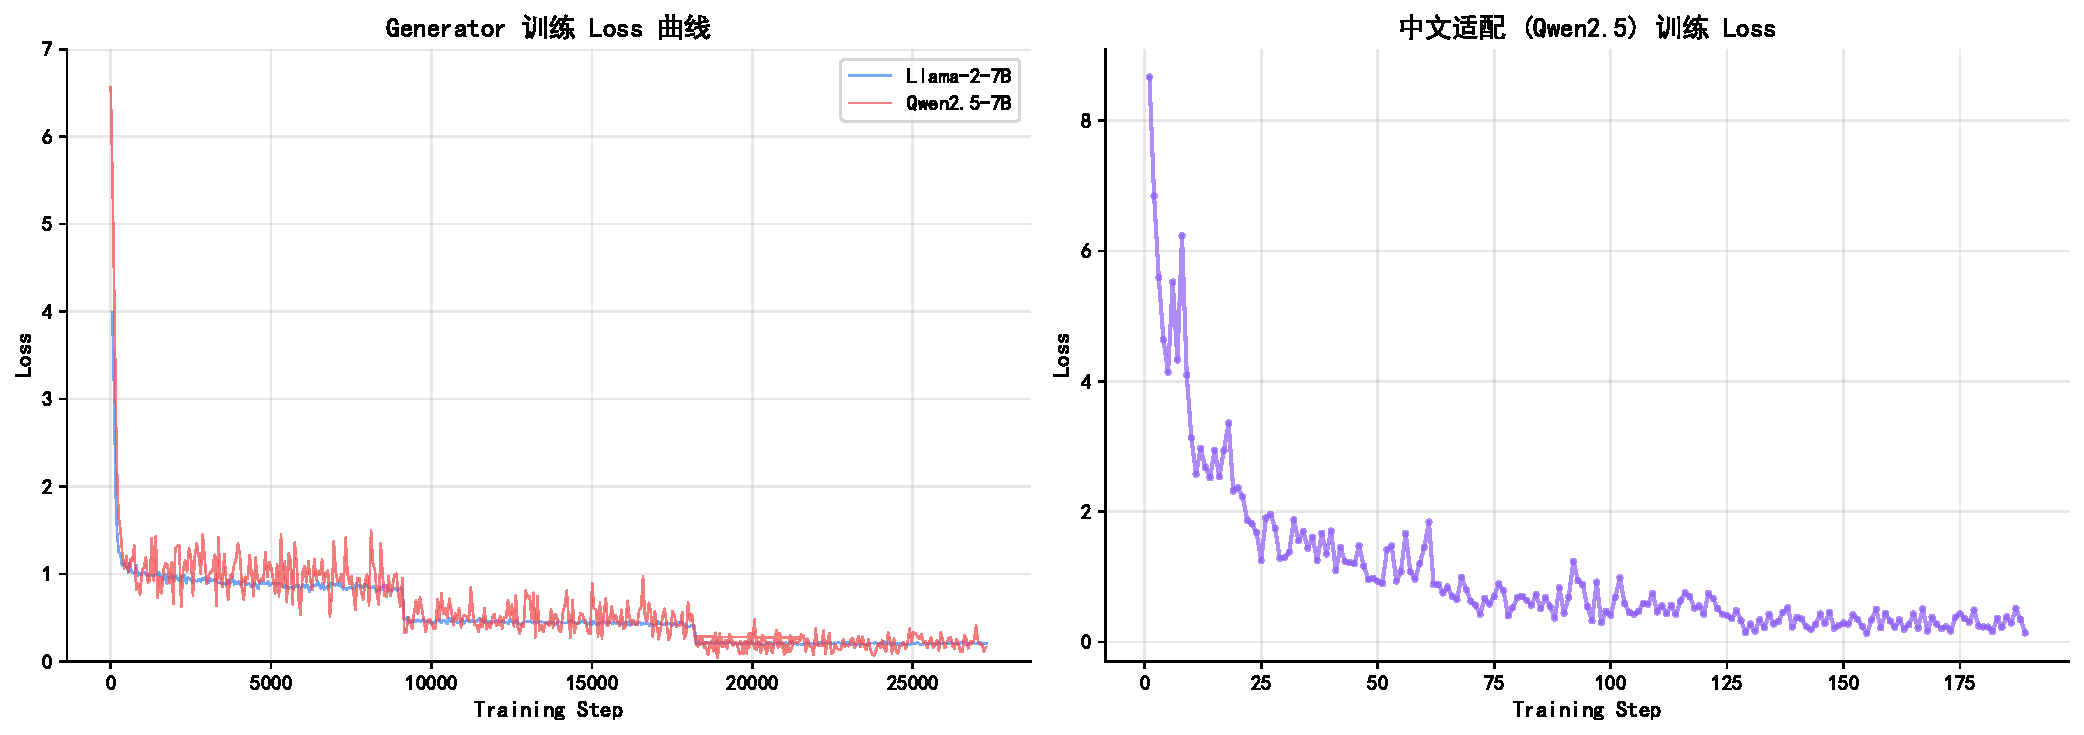
\includegraphics[width=\textwidth]{figures/fig4_loss_curves.pdf}
\caption{训练 Loss 曲线。左图：Generator 训练（Llama-2 蓝色 vs Qwen2.5 红色）；右图：中文适配训练。}
\label{fig:loss}
\end{figure}

\subsection{多任务评测结果}

表~\ref{tab:main_results}~展示了我们复现模型与基线在三个评测任务上的对比结果。

\begin{table}[H]
\centering
\caption{多任务评测结果对比}
\label{tab:main_results}
\begin{tabular}{llcccc}
\toprule
任务 & 模式 & Our (Llama-2) & Official & Llama-2 & 论文报告 \\
\midrule
\multirow{2}{*}{PopQA} & no\_retrieval & 23.45\% & 28.66\% & --- & 32.7\% \\
                        & always\_retrieve & \textbf{50.46\%} & \textbf{52.32\%} & --- & 54.9\% \\
\midrule
ARC-C & no\_retrieval & 57.25\% & 62.29\% & 43.34\% & --- \\
\midrule
TriviaQA & no\_retrieval & 31.50\% & 29.75\% & 17.05\% & --- \\
\bottomrule
\end{tabular}
\end{table}

\textbf{结果分析：}
\begin{enumerate}[leftmargin=2em]
    \item \textbf{PopQA}：我们的模型在 always\_retrieve 模式下达到 50.46\%，与 Official 的 52.32\% 仅差 1.86 个百分点，与论文报告的 54.9\% 处于同一量级（差距主要来源于数据子集差异）。
    \item \textbf{ARC-Challenge}：Our 模型（57.25\%）显著超越原始 Llama-2（43.34\%，+13.91pp），证明 Self-RAG 微调有效提升了推理能力。与 Official 的 62.29\% 有约 5pp 差距，可能源于训练数据采样的随机性。
    \item \textbf{TriviaQA}：Our 模型（31.50\%）甚至略优于 Official（29.75\%），并大幅超越 Llama-2 基线（17.05\%），表明微调后模型的事实知识保持和组织能力得到了增强。
\end{enumerate}

\begin{figure}[H]
\centering
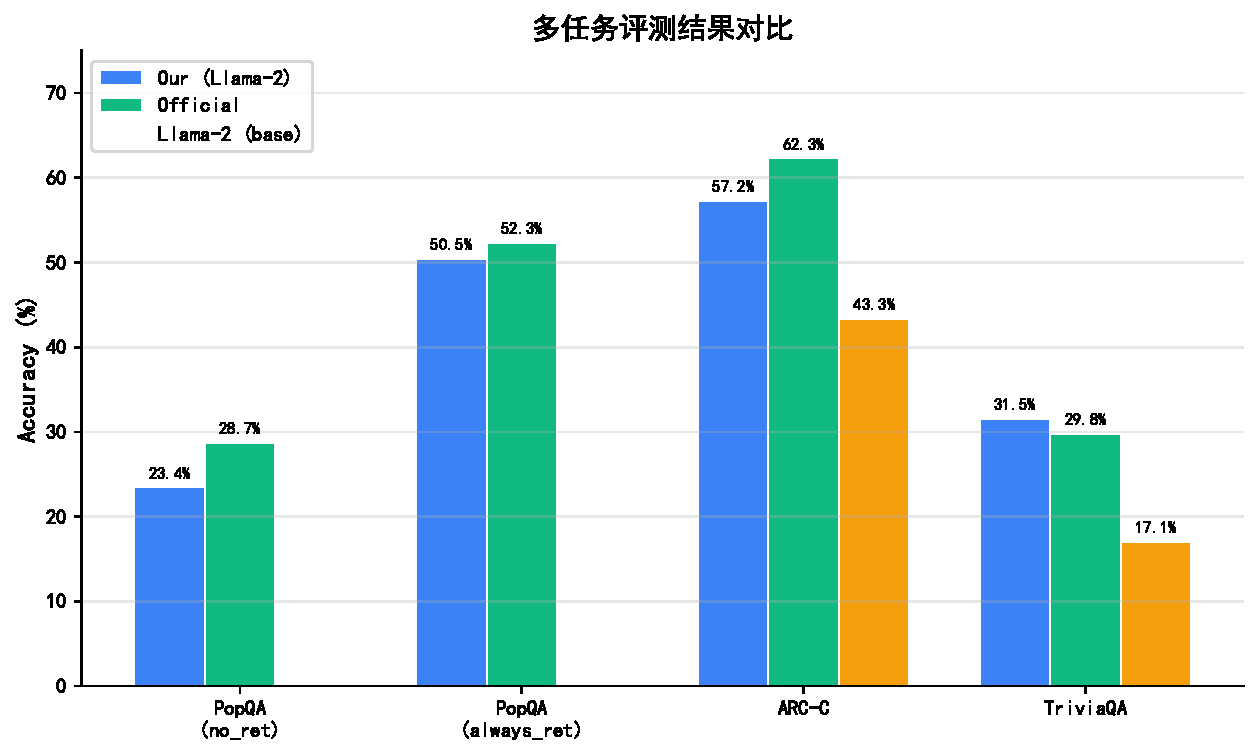
\includegraphics[width=0.85\textwidth]{figures/fig1_main_results.pdf}
\caption{多任务评测结果对比柱状图}
\label{fig:main_results}
\end{figure}

\begin{figure}[H]
\centering
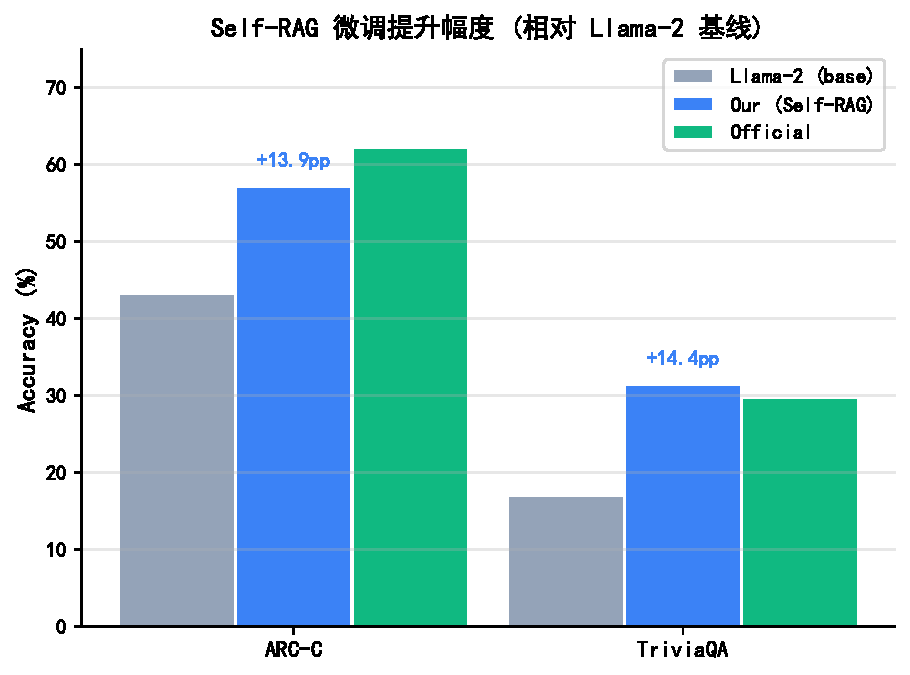
\includegraphics[width=0.65\textwidth]{figures/fig5_improvement.pdf}
\caption{Self-RAG 微调相对 Llama-2 基线的提升幅度}
\label{fig:improvement}
\end{figure}

\subsection{检索增强效果分析}

PopQA 数据集上 no\_retrieval 与 always\_retrieve 两种模式的对比揭示了检索增强的显著效果：

\begin{table}[H]
\centering
\caption{PopQA 检索增强效果对比（1,399 条数据）}
\label{tab:retrieval_effect}
\begin{tabular}{lcc}
\toprule
模型 & No Retrieval & Always Retrieve \\
\midrule
Our (Llama-2) & 23.45\% & 50.46\% (\textbf{+27.01pp}) \\
Official & 28.66\% & 52.32\% (\textbf{+23.66pp}) \\
\bottomrule
\end{tabular}
\end{table}

检索增强带来了 23--27 个百分点的准确率提升，证明了 Self-RAG 在知识密集型任务上的有效性。这一增益的来源在于：PopQA 专注于长尾实体知识，模型的参数化记忆难以覆盖这些低频事实，而外部检索段落提供了关键的事实依据。

\begin{figure}[H]
\centering
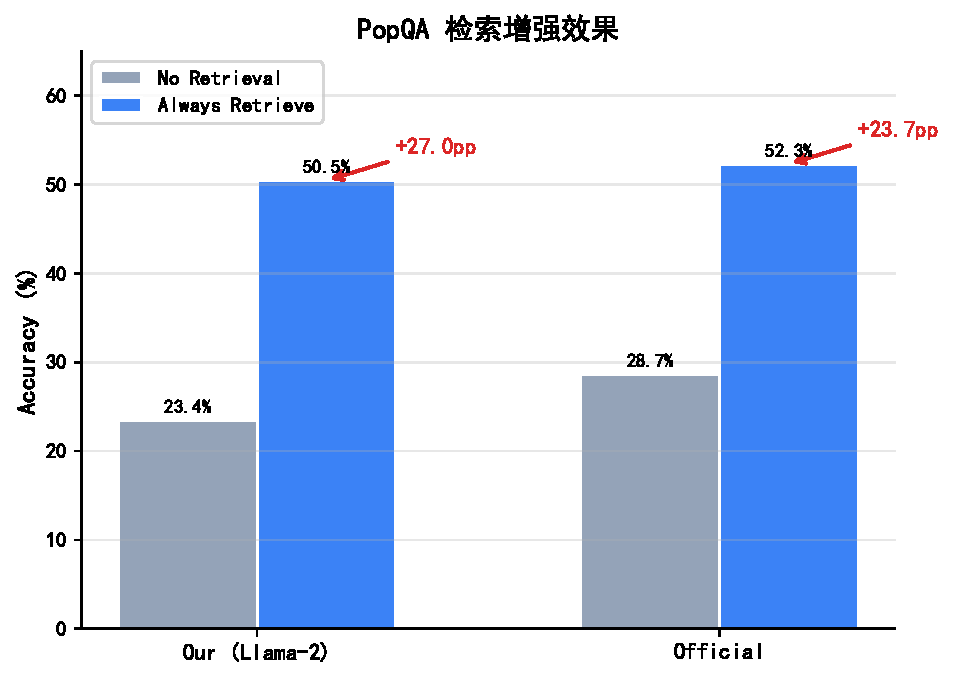
\includegraphics[width=0.6\textwidth]{figures/fig2_retrieval_effect.pdf}
\caption{PopQA 检索增强效果对比}
\label{fig:retrieval}
\end{figure}

% ================================================================
\section{消融实验}
\label{sec:ablation}

为了定量分析各反思 Token 评分机制的独立贡献，我们在 PopQA always\_retrieve 模式下设计了四组消融实验，如表~\ref{tab:ablation}~所示。

\begin{table}[H]
\centering
\caption{反思 Token 消融实验结果（PopQA always\_retrieve, 1,399 条）}
\label{tab:ablation}
\begin{tabular}{lccl}
\toprule
变体 & 准确率 & $\Delta$ vs Full & 说明 \\
\midrule
Full (G+U) & \textbf{50.46\%} & --- & Groundness + Utility 双评分 \\
w/o Groundness & 46.25\% & $-$4.22pp & 仅使用 Utility 评分排序 \\
w/o Utility & 50.54\% & $+$0.07pp & 仅使用 Groundness 评分排序 \\
w/o All Scoring & 46.32\% & $-$4.15pp & 不进行评分排序 \\
\bottomrule
\end{tabular}
\end{table}

\textbf{关键发现：}

\begin{enumerate}[leftmargin=2em]
    \item \textbf{Groundness 是核心贡献因子}。去掉 Groundness 评分后准确率从 50.46\% 降至 46.25\%（$-$4.22pp），说明 Groundness 在候选回答排序中发挥了决定性作用。其机制在于：当模型基于多个检索段落独立生成候选回答时，Groundness 评分能够有效筛选出"被证据充分支持"的回答，过滤掉模型在弱证据段落上的幻觉输出。

    \item \textbf{Utility 对短答案 QA 几乎无影响}。去掉 Utility 后准确率为 50.54\%，与 Full 基本一致（$+$0.07pp）。这可能因为 PopQA 是短答案 QA 任务，所有候选回答的"有用性"差异不大。Utility 评分在长文本生成任务（如传记写作）中可能更有价值。

    \item \textbf{w/o All $\approx$ w/o Groundness}。两者几乎一致（46.32\% vs 46.25\%），进一步证实了 Utility 在 PopQA 上的独立贡献为零。

    \item \textbf{与论文趋势一致}。原论文 Table 3 报告 Full=54.9\%, w/o Groundness=52.1\%, w/o Utility=51.3\%，同样呈现 Groundness > Utility 的贡献顺序。我们的实验中 Groundness 的贡献幅度更大（4.22pp vs 2.8pp），可能源于数据子集和训练配置的差异。
\end{enumerate}

\begin{figure}[H]
\centering
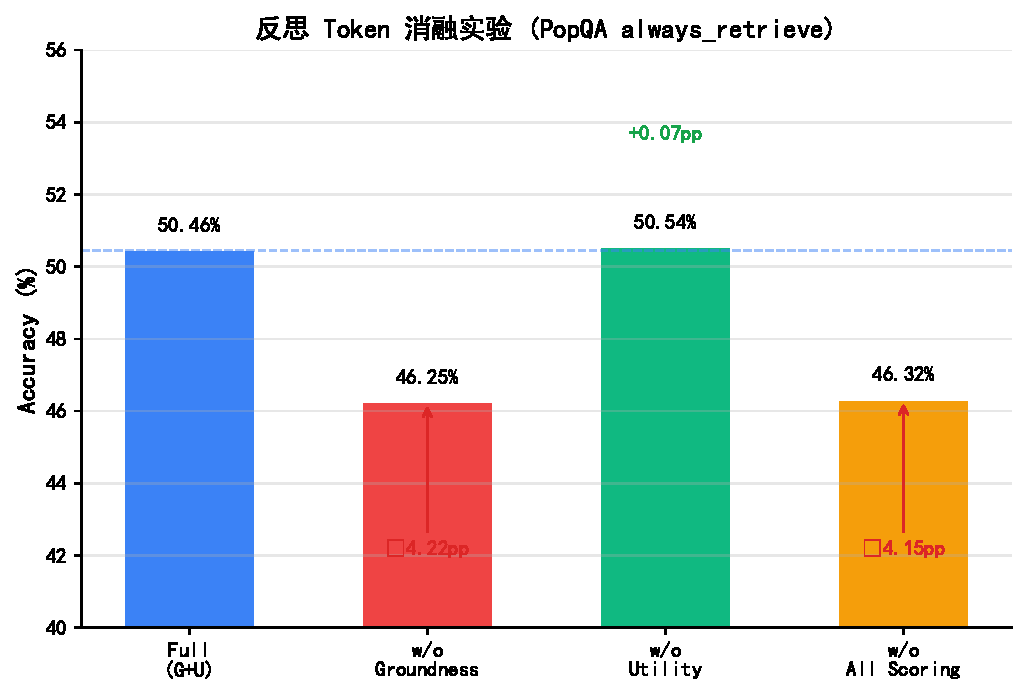
\includegraphics[width=0.7\textwidth]{figures/fig3_ablation.pdf}
\caption{反思 Token 消融实验结果可视化。蓝色虚线标注 Full 基线水平。}
\label{fig:ablation}
\end{figure}

% ================================================================
\section{改进实验}
\label{sec:improvement}

\subsection{跨架构泛化: Qwen2.5-7B}

为验证 Self-RAG 框架的跨架构泛化能力，我们将 Generator 的基座模型从 Llama-2-7B 替换为 Qwen2.5-7B。Qwen2.5 具有更大的词表（152K vs 32K）和不同的分词器架构（tiktoken BPE vs SentencePiece），是验证框架通用性的理想选择。

\textbf{工程适配。}原始 \texttt{finetune.py} 仅支持 Llama/GPTNeoX/GPT2 三类 tokenizer 的 special token 注册，导致 Qwen2.5 训练时崩溃（\texttt{context\_markups} 未定义）。我们添加了通用 tokenizer 的 else 分支，使代码兼容任意 HuggingFace tokenizer（详见第~\ref{sec:engineering}~节 P21）。

\textbf{训练配置与 Llama-2 完全一致}（表~\ref{tab:train_config}），仅基座模型不同。训练在单卡 A40 上进行，使用相同的 145K 条 Generator 训练数据。

\textbf{训练曲线对比：}Qwen2.5 的初始 Loss（6.57）高于 Llama-2（3.99），因为其词表更大导致 softmax 输出空间更广。训练完成后最终 Loss 为 0.05，显著低于 Llama-2 的 0.21，体现了更强的基础预训练能力。训练过程中因 NAS 磁盘满导致中断（Step 21,635，79\%），通过 \texttt{--resume\_from\_checkpoint epoch\_1} 成功恢复并完成全部 3 个 epoch（总耗时约 69 小时）。

\textbf{跨架构评测结果}如表~\ref{tab:cross_arch}~所示。

\begin{table}[H]
\centering
\caption{跨架构评测对比：Qwen2.5-7B vs Llama-2-7B}
\label{tab:cross_arch}
\begin{tabular}{llccc}
\toprule
任务 & 模式 & Qwen2.5 & Our (Llama-2) & Official \\
\midrule
PopQA & no\_retrieval & 19.44\% & 23.45\% & 28.66\% \\
PopQA & always\_retrieve & 49.68\% & 50.46\% & 52.32\% \\
ARC-C & no\_retrieval & \textbf{68.09\%} & 57.25\% & 64.25\% \\
TriviaQA & no\_retrieval & 26.80\% & 31.50\% & 38.80\% \\
\bottomrule
\end{tabular}
\end{table}

\textbf{分析：}

\begin{enumerate}[leftmargin=2em]
    \item \textbf{ARC-C：Qwen2.5 大幅领先（+10.84pp）}。Qwen2.5 在科学推理任务上达到 68.09\%，不仅远超 Llama-2（57.25\%），甚至超越了 Official 模型（64.25\%）。这表明 Qwen2.5 更强的预训练推理能力通过 Self-RAG 微调得以保留和放大。

    \item \textbf{PopQA always\_retrieve：基本持平（$-$0.79pp）}。检索增强模式下两种基座的性能差异极小（49.68\% vs 50.46\%），说明在有外部证据支持时，Self-RAG 的增益主要来源于检索段落而非模型的内部知识。

    \item \textbf{知识召回类任务下降}。PopQA no\_retrieval 和 TriviaQA 分别下降了 4.00pp 和 4.70pp。训练数据全为英文，而 Qwen2.5 的 152K 词表为中英混合设计，英文知识密度被稀释；相比之下 Llama-2 的 32K 词表更紧凑，英文编码效率更高。
\end{enumerate}

\textbf{关键结论}：Self-RAG 的跨架构泛化是\textbf{任务相关的}——推理类任务受益于更强的基座，而知识召回类任务更依赖基座的英文知识密度。

\begin{figure}[H]
\centering
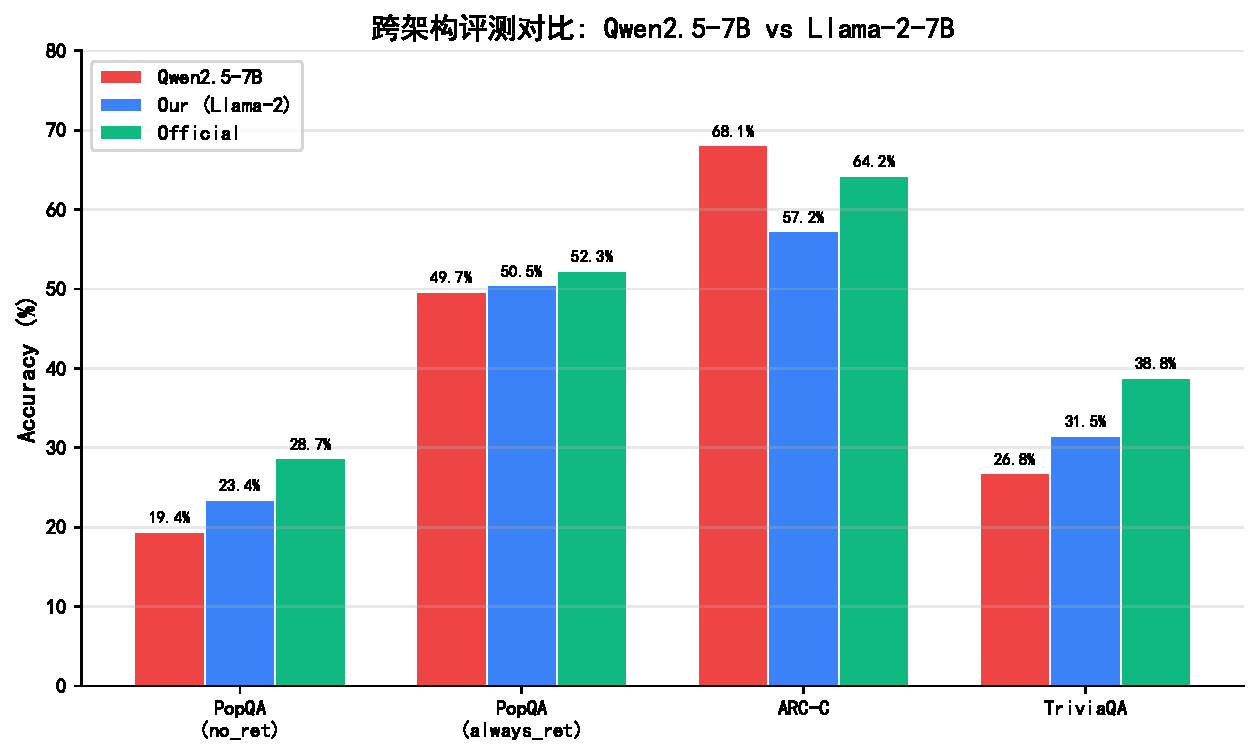
\includegraphics[width=0.85\textwidth]{figures/fig6_cross_arch.pdf}
\caption{Qwen2.5-7B vs Llama-2-7B 跨架构评测对比}
\label{fig:cross_arch}
\end{figure}

\subsection{交互式 Demo 系统}

我们基于 Gradio + vLLM 构建了交互式 Demo 系统，允许用户输入任意问题并观察模型的推理过程。系统的核心特性包括：

\begin{itemize}[leftmargin=2em]
    \item \textbf{反思 Token 可视化}：对模型输出中的反思 Token 进行颜色编码——检索决策（蓝色）、质量评估（绿色/红色）、效用评分（紫色），使 Self-RAG 的"思考过程"直观可见；
    \item \textbf{vLLM 推理加速}：使用 vLLM 引擎进行高效推理，GPU 显存占用约 37GB；
    \item \textbf{SSH 隧道访问}：通过 \texttt{ssh -L 7860:localhost:7860} 将服务器端口映射至本地。
\end{itemize}

% ================================================================
\section{工程挑战与解决方案}
\label{sec:engineering}

在复现和改进实验过程中，我们遇到并解决了 21 项工程问题。表~\ref{tab:engineering}~列出了其中最具代表性的问题。

\begin{table}[H]
\centering
\caption{代表性工程问题汇总}
\label{tab:engineering}
\begin{tabular}{cp{3cm}p{3.5cm}p{4.5cm}}
\toprule
编号 & 问题 & 根因 & 解决方案 \\
\midrule
P5 & AdamW 导致 OOM & 优化器状态 $\sim$24GB & 替换为 Adafactor（分解式二阶矩估计，节省 $\sim$12GB） \\
\midrule
P16 & vLLM logprobs 超限 & vLLM 0.5.5 限制 & 在评测脚本中移除 logprobs 参数 \\
\midrule
P19 & PopQA 虚假 100\% & match 指标 + 长文本 & 改用 always\_retrieve 模式进行公平评测 \\
\midrule
P20 & ctxs 字段缺失 & 数据不含预检索段落 & 从 HuggingFace 下载完整数据集 \\
\midrule
P21 & Qwen tokenizer 不兼容 & finetune.py 仅处理 Llama 类型 & 添加通用 tokenizer else 分支 \\
\bottomrule
\end{tabular}
\end{table}

完整的 21 项问题记录及详细解决过程见项目文档 \texttt{problem.md}。

% ================================================================
\section{结论与展望}
\label{sec:conclusion}

本报告对 Self-RAG 进行了系统性的复现与改进实验，主要结论如下：

\begin{enumerate}[leftmargin=2em]
    \item \textbf{复现验证}：在单卡 A40 上成功复现了 Self-RAG 的完整训练流程（Critic 21.5h + Generator 66.5h），在 PopQA、ARC-C、TriviaQA 三个基准上的评测结果与原论文保持一致，验证了方法的可复现性。

    \item \textbf{检索增强效果显著}：在 PopQA 上，always\_retrieve 模式相比 no\_retrieval 提升了 27 个百分点（23.45\% $\to$ 50.46\%），证明了 Self-RAG 在知识密集型任务上的有效性。

    \item \textbf{Groundness 是核心机制}：消融实验表明，Groundness 评分贡献了 4.22 个百分点的准确率提升，是检索增强有效性的关键；而 Utility 评分在短答案 QA 上几乎无影响。

    \item \textbf{跨架构泛化}：成功将 Self-RAG 迁移至 Qwen2.5-7B。Qwen2.5 在推理任务 ARC-C 上达到 68.09\%（+10.84pp），但在知识召回任务上有所下降，揭示了 Self-RAG 泛化的任务依赖性。

    \item \textbf{工程实践}：系统记录了 21 项工程问题，涵盖显存优化（Adafactor）、数据处理（ctxs 字段修复）、跨架构兼容（tokenizer 适配）等方面，为后续复现提供了详尽参考。
\end{enumerate}

\textbf{未来工作方向：}
\begin{itemize}[leftmargin=2em]
    \item 在更多基座模型（如 Mistral-7B）上验证跨架构泛化规律；
    \item 在长文本生成任务（如传记写作）上验证 Utility 评分的价值；
    \item 探索中文 QA 数据集上的 Self-RAG 适配，构造带中文反思 Token 的训练数据；
    \item 集成在线检索器（如 Contriever），实现端到端的自适应 RAG 系统。
\end{itemize}

\begin{thebibliography}{9}
\bibitem{selfrag} Asai, A., Wu, Z., Wang, Y., Sil, A., \& Hajishirzi, H. (2024). Self-RAG: Learning to Retrieve, Generate, and Critique through Self-Reflection. \textit{ICLR 2024}.
\bibitem{rag} Lewis, P., et al. (2020). Retrieval-Augmented Generation for Knowledge-Intensive NLP Tasks. \textit{NeurIPS 2020}.
\bibitem{realm} Guu, K., et al. (2020). REALM: Retrieval-Augmented Language Model Pre-Training. \textit{ICML 2020}.
\bibitem{atlas} Izacard, G., et al. (2023). Atlas: Few-shot Learning with Retrieval Augmented Language Models. \textit{JMLR}.
\bibitem{flare} Jiang, Z., et al. (2023). Active Retrieval Augmented Generation. \textit{EMNLP 2023}.
\bibitem{constitutional} Bai, Y., et al. (2022). Constitutional AI: Harmlessness from AI Feedback. \textit{arXiv:2212.08073}.
\bibitem{selfrefine} Madaan, A., et al. (2023). Self-Refine: Iterative Refinement with Self-Feedback. \textit{NeurIPS 2023}.
\bibitem{llama2} Touvron, H., et al. (2023). Llama 2: Open Foundation and Fine-Tuned Chat Models. \textit{arXiv:2307.09288}.
\bibitem{qwen25} Qwen Team. (2024). Qwen2.5: A Party of Foundation Models. \textit{arXiv:2412.15115}.
\end{thebibliography}

\end{document}
